%
% teil3.tex -- Beispiel-File für Teil 3
%
% (c) 2020 Prof Dr Andreas Müller, Hochschule Rapperswil
%
% !TEX root = ../../buch.tex
% !TEX encoding = UTF-8
%
\section{Schallausbreitung bei Überschallflugzeugen
\label{schall:section:teil3}}
\kopfrechts{Schallausbreitung bei Überschallflugzeugen}
\index{Uberschallflugzeug@Überschallflugzeug}%

In diesem Abschnitt wenden wir die in den vorherigen Abschnitten
beschriebenen Konzepte an, um die Schallausbreitung bei einem
Flugzeug im Überschall zu beschreiben.
Ziel ist es, die Entstehung des Überschallknalls herzuleiten und Strategien
\index{Uberschallknall@Überschallknall}%
zur Reduktion desselben zu verstehen.
Dabei betrachten wir eine ideale Situation, in der das Flugzeug als
Punktquelle modelliert wird.

Wir betrachten ein Flugzeug, das sich mit konstanter Geschwindigkeit
$V>0$ entlang einer horizontalen Bahn auf der Höhe $z=z_a$ über
dem Grund $z=0$ bewegt.
Das Medium sei ein ideales Gas mit örtlich variabler Temperatur
$T(z)$ aber ohne Wind, sodass
\begin{equation}
    c(z) = \sqrt{\kappa R_ST(z)} ,
    \label{eq:c-of-z}
\end{equation}
gilt. Hier ist $c(z)$ die lokale Schallgeschwindigkeit, $R_S = \frac{R}{M}$
die massenangepasste Gaskonstante und $M$ die auf der Höhe $z$ herrschende
molare Masse des Mediums.
In der Fliegerei wird die Geschwindigkeit des Flugzeugs oft über die
dimensionslose \emph{Mach-Zahl} \textit{Ma} angegeben:
\index{Mach-Zahl}%
\begin{equation}
    \textit{Ma}(z) = \frac{V}{c(z)},
    \label{eq:mach-number}
\end{equation}
wobei $\textit{Ma}<1$ Unterschall, $\textit{Ma}=1$ Schallgeschwindigkeit
und $\textit{Ma}>1$ Überschall bezeichnet.
Der Effekt des Schall- oder Mach-Kegels, welcher durch den Doppler-Effekt
\index{Mach-Kegel}
beschrieben wird, ist im Bild \ref{fig:schall:mach-zones} visualisiert.
Dabei sind die Wellenfronten als Kreise ersichtlich, die akustischen
Strahlen sind die Normalen auf den Kreisen. Die ausführliche Beschreibung
folgt in Abschnitt \ref{schall:lok-mach-emission}.

\begin{figure}
    \centering
\begin{tikzpicture}[>=latex,thick]
\clip (-6.3,-1.95) rectangle (6.3,2.4);
\node at (0,0) {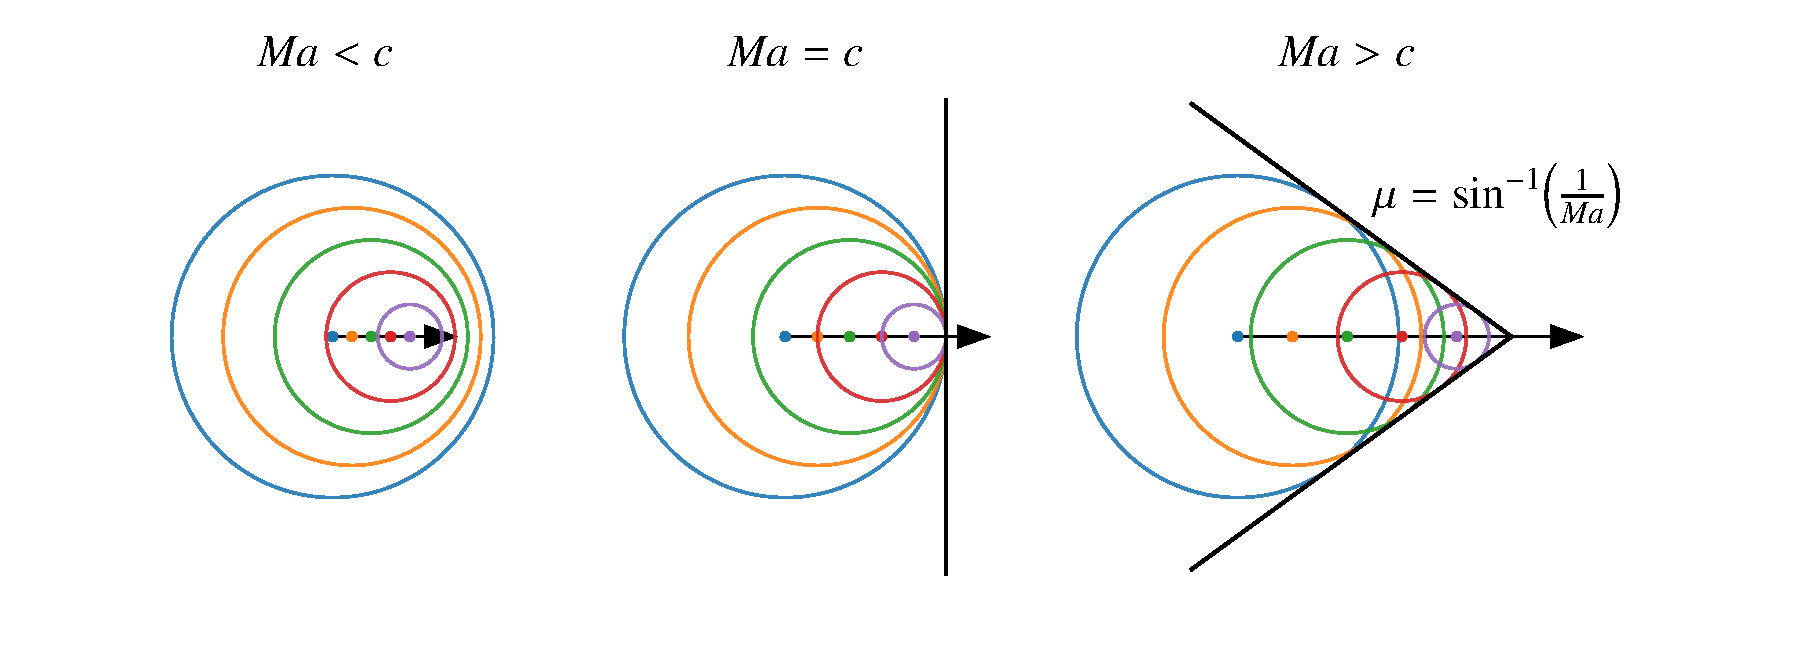
\includegraphics[width=1.14\textwidth]{papers/schall/figures/mach_doppler_triptych_offsets.pdf}};
%\fill[color=red,opacity=0.1] (-6.3,-1.95) rectangle (6.3,2.4);
\end{tikzpicture}
    \caption{Dopplereffekt bei Unterschall, Schallgeschwindigkeit und Überschall.
    Für die Schallgeschwindigkeit und den Überschall ist zusätzlich der
    Mach-Kegel mit dem Mach-Winkel $\mu$ eingezeichnet. Dabei sind die
    Wellenfronten als Kreise ersichtlich, die akustischen Strahlen sind
    die Normalen auf den Kreisen.}
    \label{fig:schall:mach-zones}
\end{figure}
Das vom Flugzeug erzeugte Schallereignis bewegt sich mit Geschwindigkeit $V$
mit dem Flugzeug, der Schall breitet sich aber mit $c(z)$ aus.
Diese ist jedoch nicht überall gleich: je dichter ein Medium ist, desto
höher ist die Schallgeschwindigkeit, was im
Abschnitt~\ref{schall:subsection:atmos-scenarios} aufgezeigt wird.
Tritt die vom Flugzeug erzeugte Schockwelle in eine Region mit höherer
Schallgeschwindigkeit ein sodass $V<c(z)$ gilt, so wird die Schockwelle
nach oben abgelenkt und kann sich nicht mehr bis zum Boden ausbreiten.
Tritt hingegen eine Schallwelle in eine Region mit niedrigerer
Schallgeschwindigkeit ein, sodass $V>c(z)$ gilt, so wird eine Schockwelle
entstehen, die sich bis zum Boden ausbreiten kann.

Wenn $Ma \gg 1$ ist, wie zum Beispiel beim Flug der Concorde mit $\textit{Ma} \approx 2.2$,
\index{Concorde}%
dann spielen die Variationen von $c(z)$ keine grosse Rolle.
Wenn aber $V$ nahe bei $c(z)$ ist, dann kommt es zu merklichen Einflüssen,
die dazu genutzt werden, den Überschallknall abzuschwächen oder zu
unterdrücken, was im Abschnitt~\ref{schall:section:boom} analysiert wird.

\subsection{Lokaler Mach-Winkel und Emissionsrichtung}
\label{schall:lok-mach-emission}
In einem homogenen Medium bildet sich der Mach-Kegel mit Halbwinkel
\begin{equation*}
    \mu = \arcsin\biggl(\frac{1}{\textit{Ma}}\biggr).
\end{equation*}
In einem geschichteten Medium setzt man diesen lokal an der
Emissionshöhe $z_a$, auf welcher das Flugzeug fliegt, an:
\begin{equation}
    \mu_a := \arcsin\biggl(\frac{1}{\textit{Ma}(z_a)}\biggr)
    = \arcsin\biggl(\frac{c(z_a)}{V}\biggr) .
    \label{eq:local-mach-angle}
\end{equation}
Der Rand des Mach-Kegels wird oft als Mach-Rand bezeichnet, welcher im
vertikalen Schnitt $(x,z)$ durch akustische Strahlen begrenzt ist.
Dies nennt man die \emph{geometrische Akustik}.

\subsubsection{Akustische Strahlen}
Seien $\tau(\boldsymbol{x})=\mathrm{const.}$ die \emph{Wellenfronten}, visualisiert
als Kreise in der Abbildung \ref{fig:schall:mach-zones}.
Die akustischen Strahlen sind ihre Normalen; formal verlaufen sie
in Richtung des Gradienten $\nabla\tau$ und beschreiben die lokale
Ausbreitungsrichtung
\[
    \dot{\boldsymbol{x}}(s) \parallel \nabla\tau(\boldsymbol{x}),\qquad
    \text{Strahl} \perp \text{Wellenfront}.
\]
In einem homogenen Medium sind Strahlen Geraden.
Für einen bewegten Punktstrahler, wie zum Beispiel ein Flugzeug,
sind die Wellenfronten die Kreise $r=c\tau$ um die jeweiligen Emissionsorte
$x=V(t-\tau)$; die Strahlen an jedem Punkt der Front zeigen radial auf den Emissionsort.

\subsubsection{Mach-Rand vs.~Strahlen}
Der \emph{Mach-Rand} ist die Einhüllende der expandierenden Wellenfronten:
\index{Wellenfront}%
die Menge aller Tangentialpunkte zwischen den Kreisen und einer Kurve.
An Einhüllendenpunkten gilt, dass der Strahl auf der Einhüllenden senkrecht
steht,
denn der Strahl ist normal auf die Wellenfront.
Die Einhüllende ist dort tangential an die Wellenfront.

\begin{itemize}
\item \textbf{Unterschall} ($\textit{Ma}<1$):
Es existiert keine Einhüllende; die Kreise überlappen, Strahlen
sind radial zu ihren Emissionszentren und es entsteht kein Mach-Rand.

\item \textbf{Schallnah} ($\textit{Ma}=1$):
Die Einhüllende degeneriert zu einer Geraden senkrecht zur Flugrichtung,
was zu einer ``vertikale'' Linie in der Visualisierung in Abbildung~\ref{fig:schall:mach-zones} führt.
Die Strahlen an den Berührungspunkten sind orthogonal zu dieser Linie,
also parallel zur Flugrichtung.
Sie liegen nicht auf der Einhüllenden, sondern stehen senkrecht zu ihr.

\item \textbf{Überschall} ($\textit{Ma}>1$):
Die Einhüllende besteht aus zwei Geraden mit Halbwinkel $\mu_a$ zur
Flugrichtung.
%Dies sind die Generatoren des Mach-Kegels, was der Mach-Rand ist,
%und nicht die Strahlen selbst.
Die Strahlen in den Berührungspunkten stehen senkrecht zu
diesen Linien und zeigen radial zu ihren jeweiligen Emissionszentren;
sie verlaufen nicht entlang der Mach-Linien.
\end{itemize}

\subsection{Strahlen in geschichtetem Medium}
Für isotrope, ruhende Medien mit $c=c(z)$ liefert die geometrische
Akustik eine Snell-ähnliche Invariante:
\begin{equation}
  \frac{\sin\psi(z)}{c(z)} = \text{const} =: K ,
  \label{eq:snell-acoustics}
\end{equation}
wobei $\psi(z)$ der Winkel des Strahls gegen die Vertikale
(Schichtnormale) und $\mu(z)=90^\circ-\psi(z)$ der Winkel gegen
die Horizontale ist.
Wählt man als Anfangsbedingung den lokalen Mach-Winkel an $z=z_a$,
also $\psi(z_a)=90^\circ-\mu_a$, dann folgt aus
\eqref{eq:local-mach-angle} und \eqref{eq:snell-acoustics}
\[
  K = \frac{\sin(90^\circ-\mu_a)}{c(z_a)} =
  \frac{\cos\mu_a}{c(z_a)} =
  \frac{\sqrt{1-\bigl(c(z_a)/V\bigr)^2}}{c(z_a)}.
\]
Damit ist für Mach-Strahlen die Invariante
\begin{equation}
  K = \frac{\sqrt{1-\bigl(c(z_a)/V\bigr)^2}}{c(z_a)}.
  \label{eq:K-from-mu}
\end{equation}
Mit $\tan\psi = \dfrac{dx}{dz}$, $\sin\psi(z) = Kc(z)$ und
$\cos\psi(z) = \sqrt{1 - K^2 c^2(z)}$ erhält man
\begin{equation*}
  \frac{dz}{dx} = \cot\psi(z) =
  \frac{\cos\psi(z)}{\sin\psi(z)} =
  \frac{\sqrt{1 - K^2 c^2(z)}}{Kc(z)}.
\end{equation*}
Einsetzen von \eqref{eq:K-from-mu} liefert die
Differentialgleichung der Mach-Ränder:
\[
  \frac{dz}{dx} = \frac{\sqrt{1 - \bigl(c(z)/V\bigr)^2}}{c(z)/V}
  = \sqrt{\frac{V^2}{c^2(z)} - 1},
\]
oder äquivalent
\begin{equation}
  \frac{dx}{dz} = \frac{1}{\sqrt{\frac{V^2}{c^2(z)} - 1}} =
  \frac{c(z)}{\sqrt{V^2 - c^2(z)}},
  \label{eq:ray-ode-inverse}
\end{equation}
mit Anfangsbedingung $x(z_a)=0$ senkrecht unter dem Flugzeug.
Die Lösungen von \eqref{eq:ray-ode-inverse} geben die gekrümmten Stossränder
im $(x,z)$-Schnitt.
Die Bedingung für reale Strahlen ist $V>c(z)$
entlang der Bahn; wo $V=c(z)$, existiert ein Wendepunkt/kritische Höhe
(horizontale Tangente), darunter eine \emph{Schattenzone}.
\index{Schattenzone}%
Dies wird in Abschnitt~\ref{schall:subsection:atmos-scenarios} genauer analysiert.

\subsection{Boom-Teppich am Boden}
Die horizontale Entfernung vom Lotpunkt des Flugzeugs bis zum
Aufprallpunkt eines Strahls am Boden ($z=0$) ergibt sich bei einfachem
Fall (kein Wind, keine lateralen Gradienten) durch die
Integration von \eqref{eq:ray-ode-inverse} und bildet den Boom-Teppich:
\begin{equation}
    \quad
    x_g = \int_{0}^{z_a} \frac{c(\zeta)}{\sqrt{V^2 - c^2(\zeta)}} \,d\zeta,
    \qquad \text{sofern } V>c(\zeta) \text{ für } \zeta\in[0,z_a].
    \quad
    \label{eq:ground-range}
\end{equation}
In einer Schicht mit $V\le c(\zeta)$, wird der Mach-Rand kontinuierlich
nach oben abgelenkt und die Schockwelle breitet sich nicht weiter aus,
was zu Schattenzonen am Boden führt.

\subsection{Atmosphären-Szenarien}\label{schall:subsection:atmos-scenarios}
Wir modellieren $T(z)$ stückweise linear und mit trockener
Standardatmosphäre ohne Wind, woraus $c(z)$ via \eqref{eq:c-of-z} folgt.
Die drei grundlegenden Szenarien sind: Normale Lage, Inversionslage und
Wendepunkt mit Bodenschatten.
Die Abbildungen \ref{fig:schall:norm-lage} und \ref{fig:schall:inv-lage}
zeigen die Schallausbreitung für die Szenarien normale Lage
\eqref{eq:normal-lapse} und Inversionslage \eqref{eq:inversion}.
Die Abbildung \ref{fig:schall:norm-vs-inv-lage} stellt beide Szenarien
direkt gegenüber.
Dabei sieht man, dass die Ausbreitung der Schallwellen
in der normalen Lage nach oben gebogen wird (oben ist $c$ kleiner),
während sie in der Inversionslage nach unten gebogen wird (unten ist $c$ kleiner).

\subsubsection{Normale Lage}
Bei der normalen Lage nimmt die Temperatur mit der Höhe ab,
wie es tagsüber über einem warmen Boden üblich ist.
Es gelte
\begin{equation}
    T(z) = T_0 - Lz \quad (L>0),
    \qquad
    c(z) = \sqrt{\kappa R\,(T_0 - Lz)} .
    \label{eq:normal-lapse}
\end{equation}
Da $c$ mit $z$ abnimmt, sind höhere Schichten akustisch
``langsamer''; Strahlen werden zum langsameren Bereich hin
gebogen, d.~h.~nach oben.
Damit nimmt $x_g$ in \eqref{eq:ground-range} ab, was sich in einem Anheben
der Strahlen widerspiegelt, und es können \emph{Bodenschatten}
entstehen, wenn in Bodennähe $V\lesssim c(0)$ ist.

\subsubsection{Inversionslage}
Bei der Inversionslage nimmt die Temperatur mit der Höhe zu, was bei klarem
Himmel in der Nacht über einem kalten Boden vorkommen kann.
Es gelte
\begin{equation}
    T(z) = T_0 + L_{I} z \quad (L_{I}>0),
    \qquad
    c(z) = \sqrt{\kappa R(T_0 + L_{I} z)} .
    \label{eq:inversion}
\end{equation}
Nun nimmt $c$ mit $z$ zu; höhere Schichten sind akustisch ``schneller''.
Strahlen biegen daher nach unten und werden zum Boden zurückgeführt.
Dadurch wächst $x_g$ in \eqref{eq:ground-range} und der Überschall
kann weiter getragen werden, was zu weniger oder bis zu keine
Schattierung am Boden führt.
Gleichzeitig verschlankt sich der Boom-Teppich, was die
Lärmbelastung in der Mitte erhöht.

\subsubsection{Wendepunkt und Bodenschatten}
Tritt irgendwo im Intervall $[0,z_a]$ ein Bereich auf, in dem
$V\le c(\zeta)$ gilt, so existiert eine
kritische Höhe $z_\ast\in(0,z_a]$ mit
\begin{equation}
    c(z_\ast)=V.
    \label{eq:turning-def}
\end{equation}
Dieser kritische Punkt ist ein Wendepunkt des akustischen Ausbreitungsstrahls.
Aus der Strahlgleichung \eqref{eq:ray-ode-inverse} folgt, dass der
Integrand für $z\to z_\ast$ gegen $\boldsymbol{\infty}$ geht und für $z<z_\ast$ imaginär würde.
Der Strahl besitzt bei $z=z_\ast$ eine horizontale Tangente und kehrt um;
er kann die Schicht $z<z_\ast$ nicht durchdringen.
Die maximale horizontale Ausbreitung bis zum Wendepunkt ist gegeben durch
\begin{equation}
    x_{\mathrm{turn}}
    = \int_{z_\ast}^{z_a} \frac{c(\zeta)}{\sqrt{V^2 - c^2(\zeta)}}\,d\zeta,
    \label{eq:x-turn}
\end{equation}
was in Abbildung \ref{fig:schall:norm-lage} für $\textit{Ma}=1.05$ ersichtlich ist.
Der Bereich unterhalb der Wendeschicht $z<z_\ast$ liegt somit in einer
Schattenzone, in der man keinen Überschallknall des Flugzeugs hören kann.
Für streng monotone Profile entscheidet die einfache Bedingung
\begin{equation}
    \text{Bodentreffer existiert} \quad\Leftrightarrow\quad V>c(z)\quad\forall\,z\in[0,z_a].
    \label{eq:ground-hit-condition}
\end{equation}

\begin{figure}
    \centering
\begin{tikzpicture}[>=latex,thick]
\clip (-6.3,-3.6) rectangle (6.3,3.25);
\node at (-0.35,0) {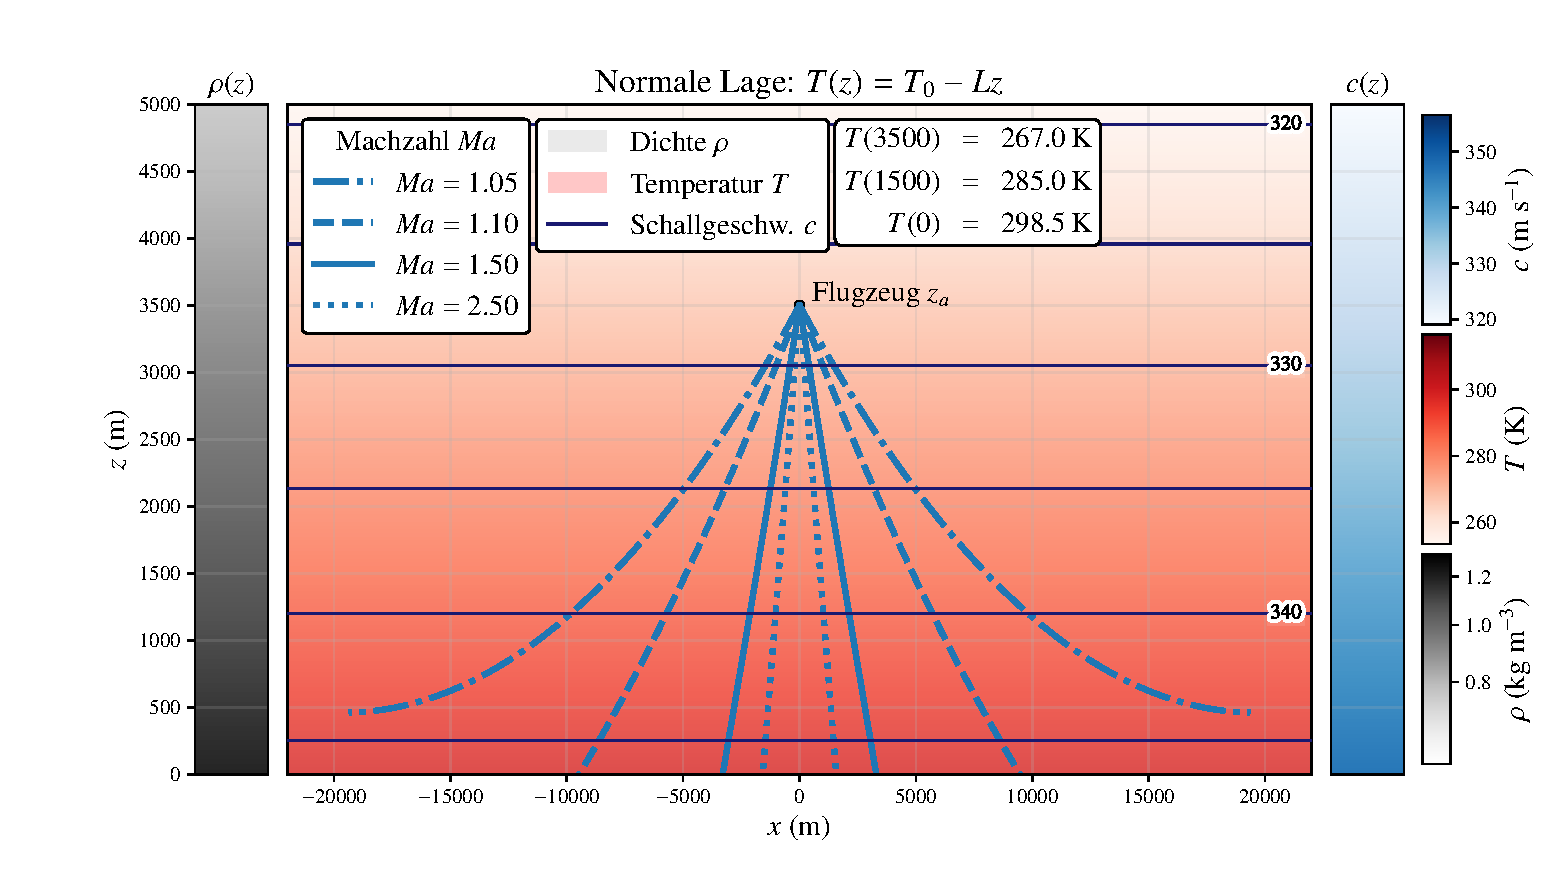
\includegraphics[width=1.09\textwidth]{papers/schall/figures/normal_sidepanels.pdf}};
%\fill[color=red,opacity=0.1] (-6.3,-4) rectangle (6.3,4);
\end{tikzpicture}
    \caption{Mach-Randausbreitung für eine normale Lage. Die Mach-Zahl
    ist konstant auf der Höhe des Flugzeugs $z_a=3\,500 m$ gesetzt für
    $\textit{Ma} \in \{1.05, 1.1, 1.5, 2.5 \}$.
    Die Temperatur ist $T(1500\,\mathrm{m}) = 285.0\,\mathrm{K}$ gegeben mit einem
    linearen Abfall von $9\,\mathrm{K/km}$.
    Je langsamer das Flugzeug, desto grösser ist der Ausbreitungswinkel
    $\mu_a$, desto stärker die Ablenkung nach oben und desto grösser
    die horizontale Reichweite $x_g$.
    Dies gilt bis $V\le c(z)$ und der kritische Punkt erreicht wird,
    sodass die Schattenzone beginnt und die Schockwelle nicht den
    Boden erreicht.}
    \label{fig:schall:norm-lage}
\end{figure}

\begin{figure}
    \centering
\begin{tikzpicture}[>=latex,thick]
\clip (-6.3,-3.6) rectangle (6.3,3.25);
\node at (-0.35,0) {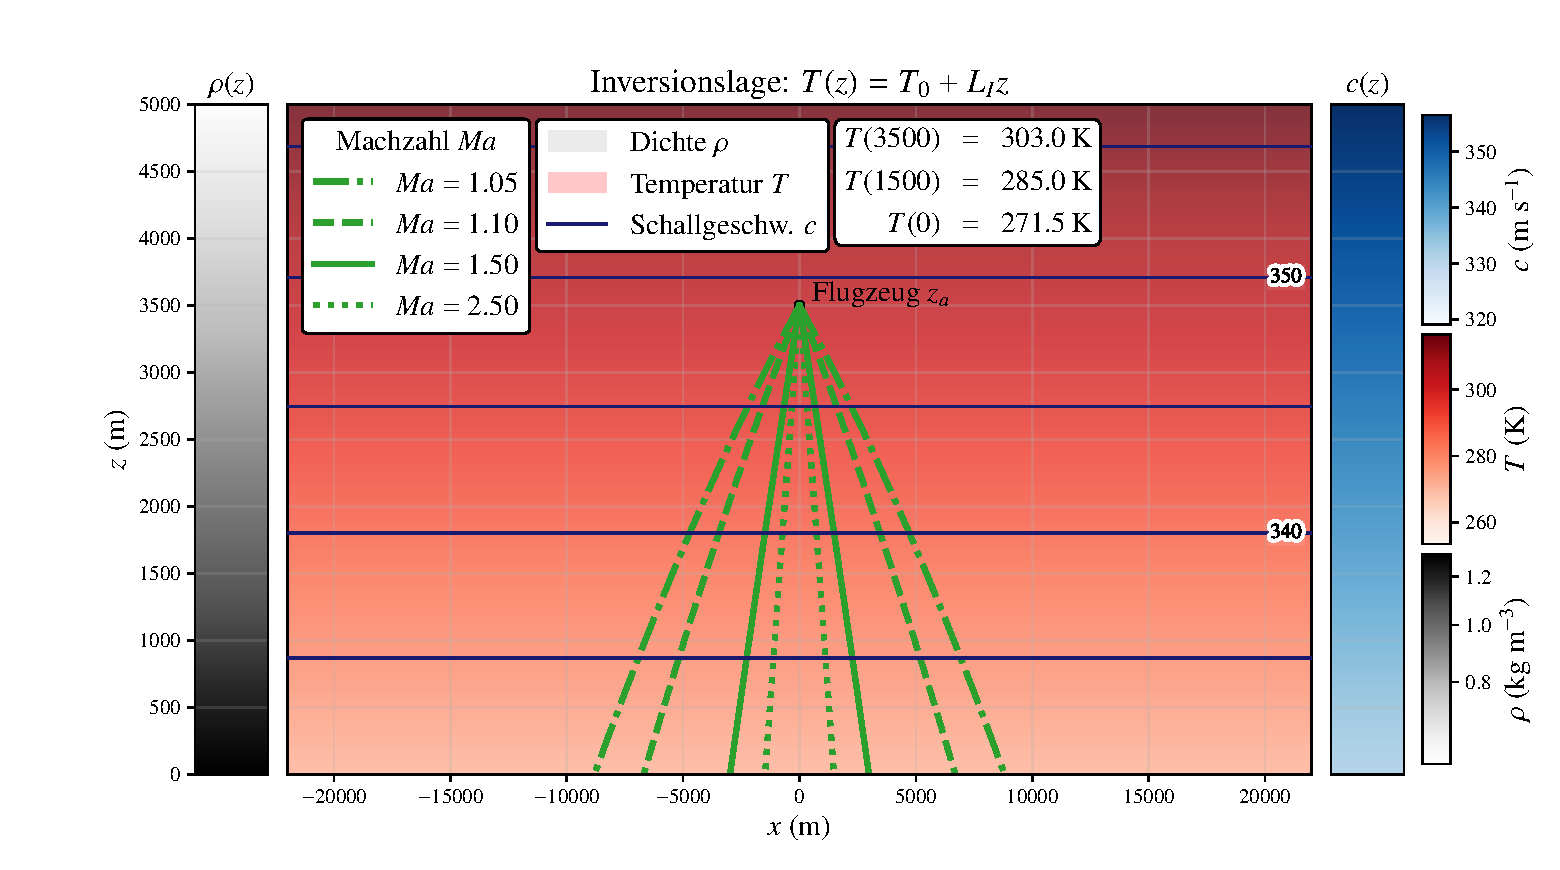
\includegraphics[width=1.09\textwidth]{papers/schall/figures/inversion_sidepanels.pdf}};
%\fill[color=red,opacity=0.1] (-6.3,-4) rectangle (6.3,4);
\end{tikzpicture}
    \caption{Mach-Randausbreitung für eine Inversionslage. Die Mach-Zahl
    ist konstant auf der Höhe des Flugzeugs $z_a=3\,500 m$ gesetzt für
    $\textit{Ma} \in \{1.05, 1.1, 1.5, 2.5 \}$.
    Die Temperatur ist $T(1500\,\textrm{m}) = 285.0\,\mathrm{K}$ gegeben mit einer
    linearen Zunahme von $9\,\mathrm{K/km}$.
    Je langsamer das Flugzeug, desto grösser ist der Ausbreitungswinkel
    $\mu_a$, desto stärker die Ablenkung nach unten und desto
    grösser die horizontale Reichweite $x_g$.}
    \label{fig:schall:inv-lage}
\end{figure}

\begin{figure}
    \centering
\begin{tikzpicture}
\clip (-6.3,-2.95) rectangle (6.3,2.95);
\node at (-0.015,0) {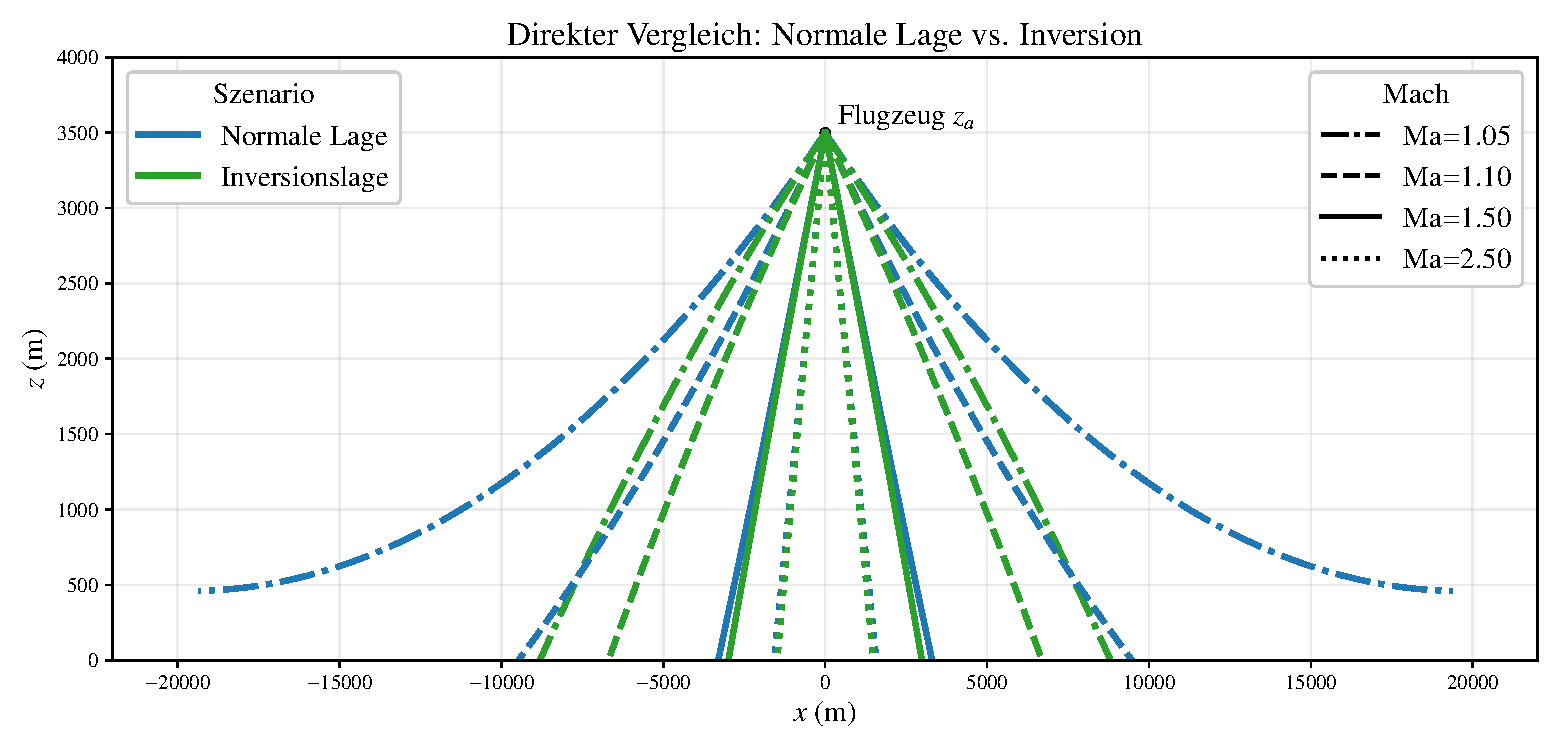
\includegraphics[width=1.027\textwidth]{papers/schall/figures/overlay_clean.pdf}};
%\fill[color=red,opacity=0.1] (-6.3,-4) rectangle (6.3,4);
\end{tikzpicture}
    \caption{Die Mach-Randausbreitung im direkten Vergleich zwischen
    normaler Lage und Inversion. Die Eigenschaften der beiden Szenarien
    sind identisch zu den Abbildungen \ref{fig:schall:norm-lage}
    und \ref{fig:schall:inv-lage}.}
    \label{fig:schall:norm-vs-inv-lage}
\end{figure}
